% This is the section of the results focused on the assembly


\chapter{Transcriptome Assembly}

\section{Assembly Quality}

\subsection{Quality Statistics}


A primary motivation for the assembly and subsequent annotation has been the amount of data(reads) that are accounted for in the existing/reference annotation. An average of 1.7 million reads per sample are accounted for in these regions, out of an average of 10[M]illion rRNA-free reads.  Only 17\% of the usable, quality data are accounted for by the coding sequences of the reference annotation. However, 10M reads exceeds the typical sample depth for comparable efforts of transcript boundary identification. For these reasons, transcriptome assembly is necessary for transcript boundary identification.

4177 transcripts (7.18Mb from a 8.3Mb genome) were assembled, after removing duplicates. Each of these transcripts aligned to one location in the genome with \textgreater 98\% identity and less than 30bp of gaps. Of these, 1057 transcripts spanning 4.56Mb (25\% by the number of assembled transcripts;  63.5\% by assembled basepairs) contain 3287(86\%) reference ORF or one of 60 novel CDSes.  The remaining 3120 (75\% by number, 36.5\% by basepairs) of transcripts are novel (Fig. 1. Orange) and their lengths range from 200-32.7kb. The reference-ORF containing transcripts will be referred throughout as the ``standard'' set of transcripts and most of the investigation below describes this group.

The standard set of transcripts were larger on average by approximately an order of magnitude.

\begin{comment}



\begin{figure}
\begin{center}
\begin{minipage}[b]{2.25in}
\resizebox{2.25in}{2.5in}{
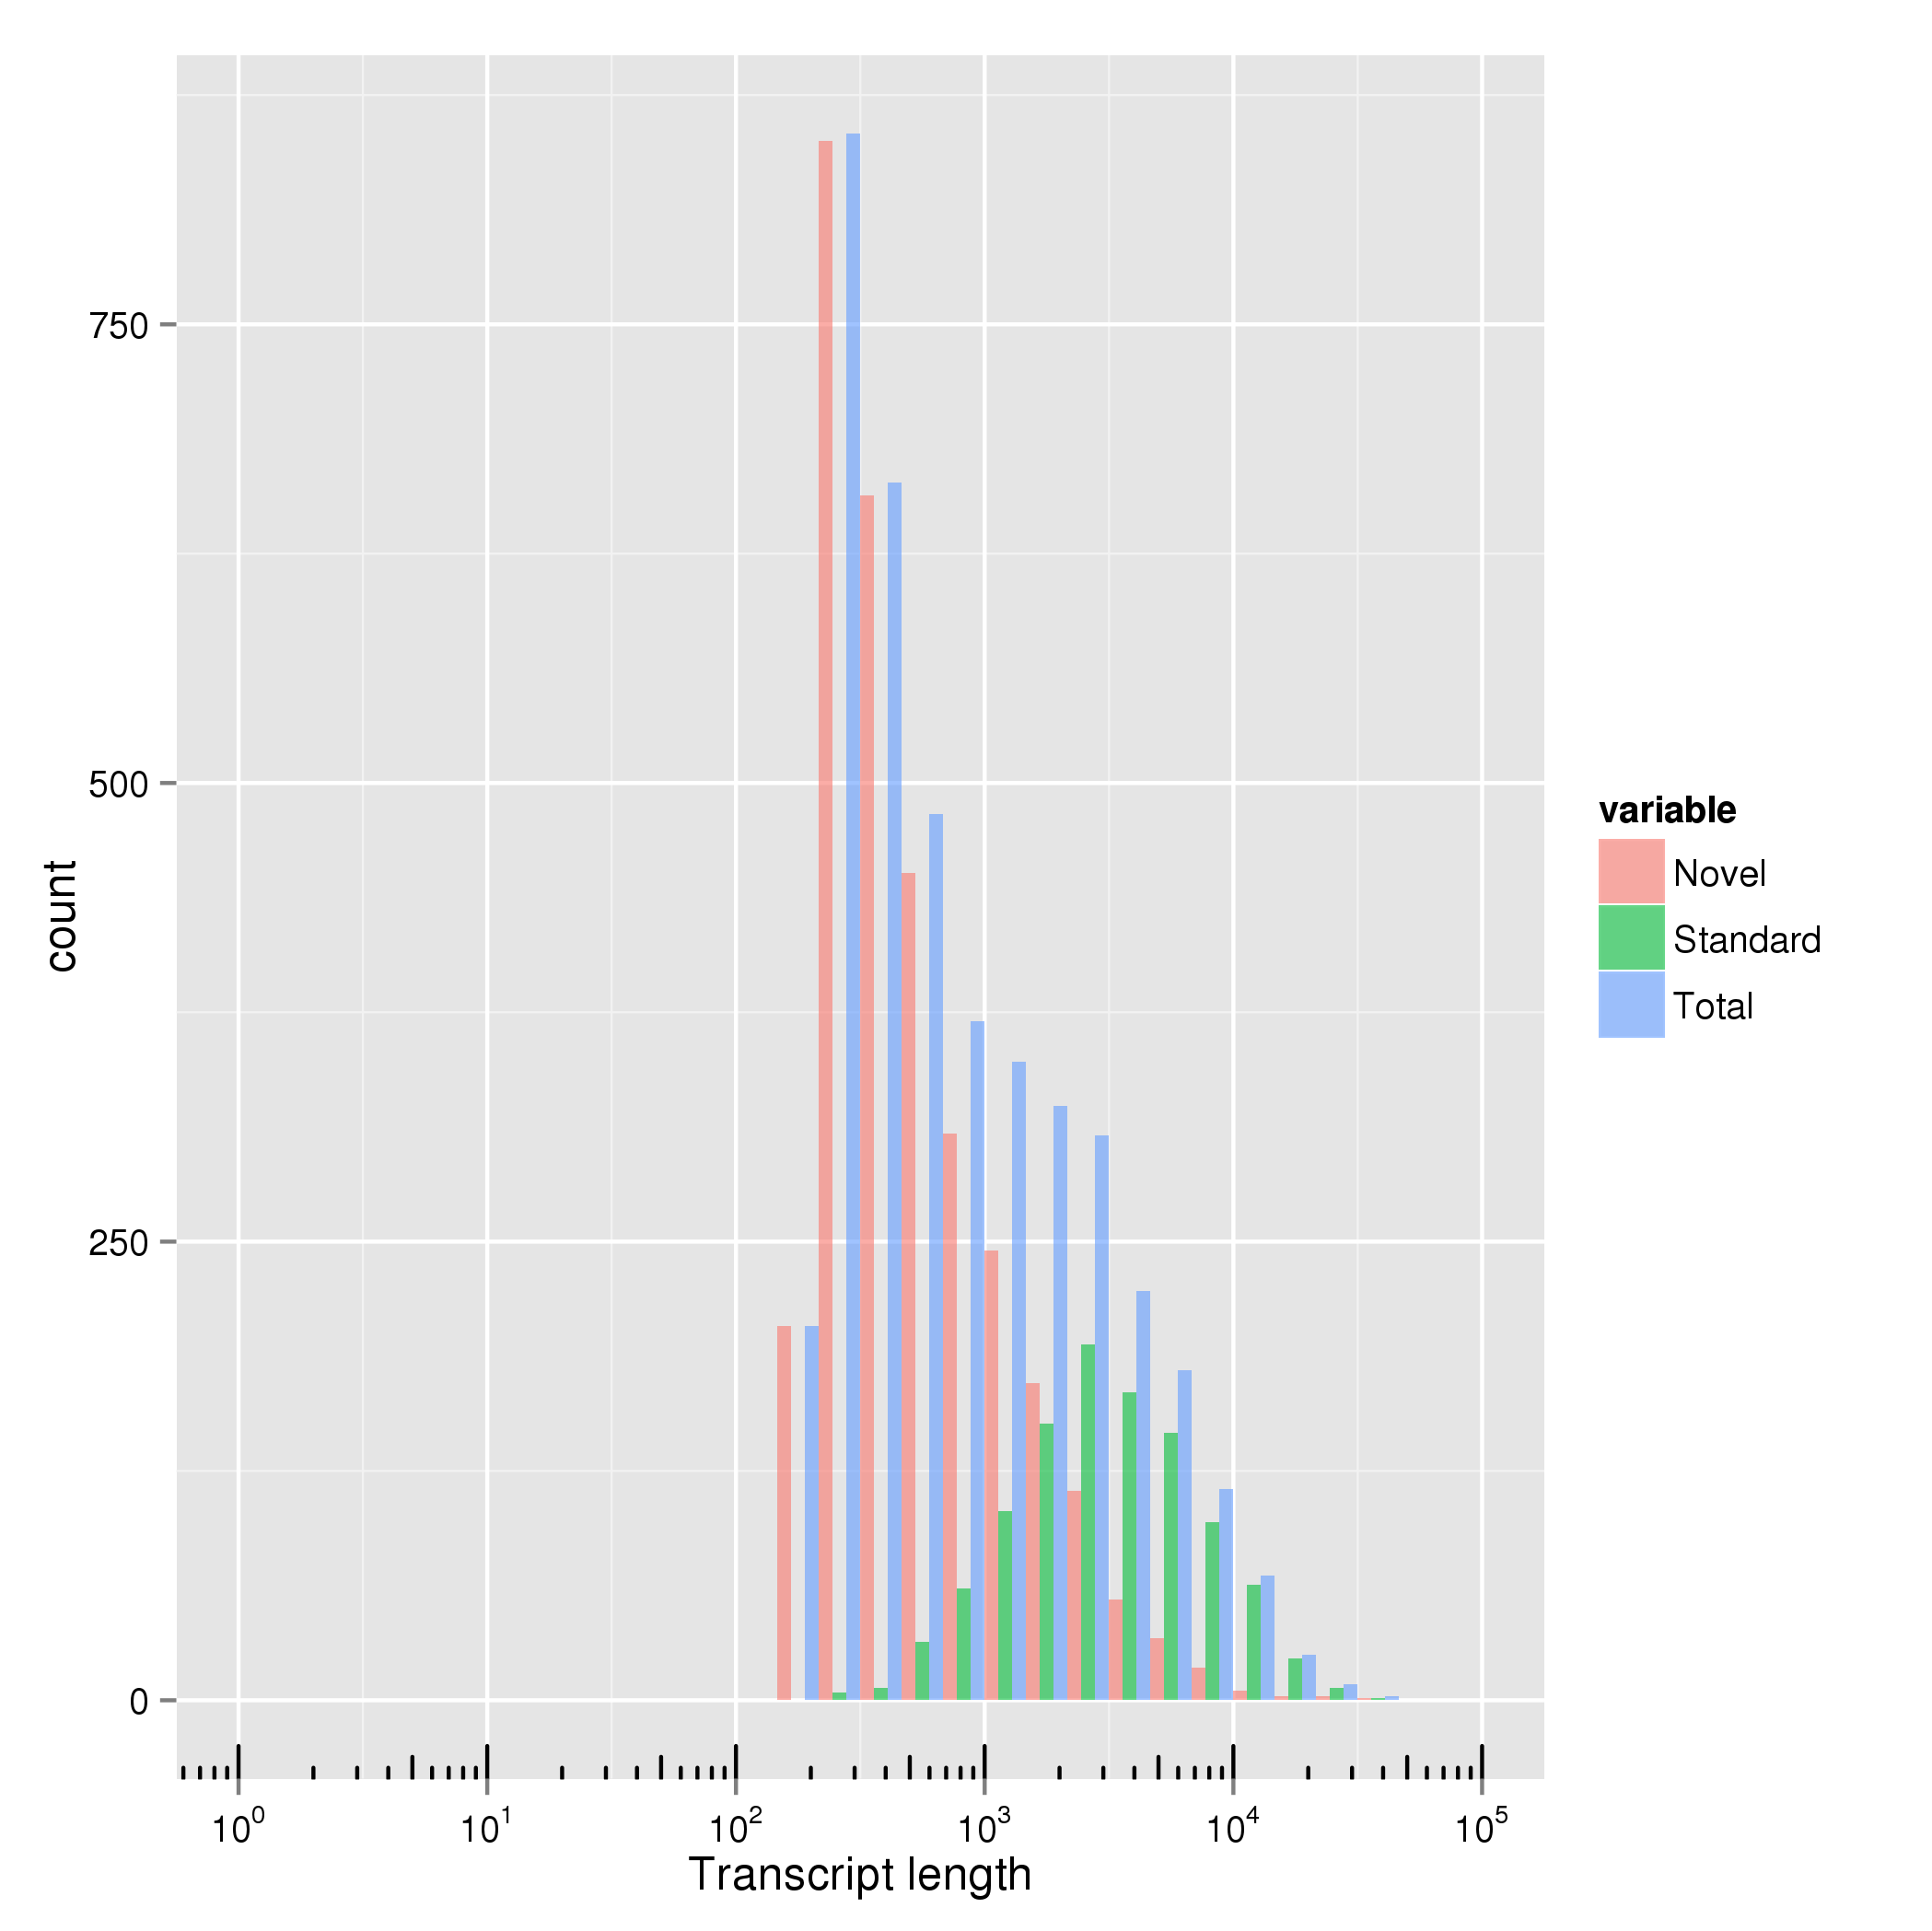
\includegraphics{images/Assembly/Summary/ftranscript_length.png}
}
\end{minipage}
\begin{minipage}[b]{2.25in}
\resizebox{2.25in}{2.5in}{
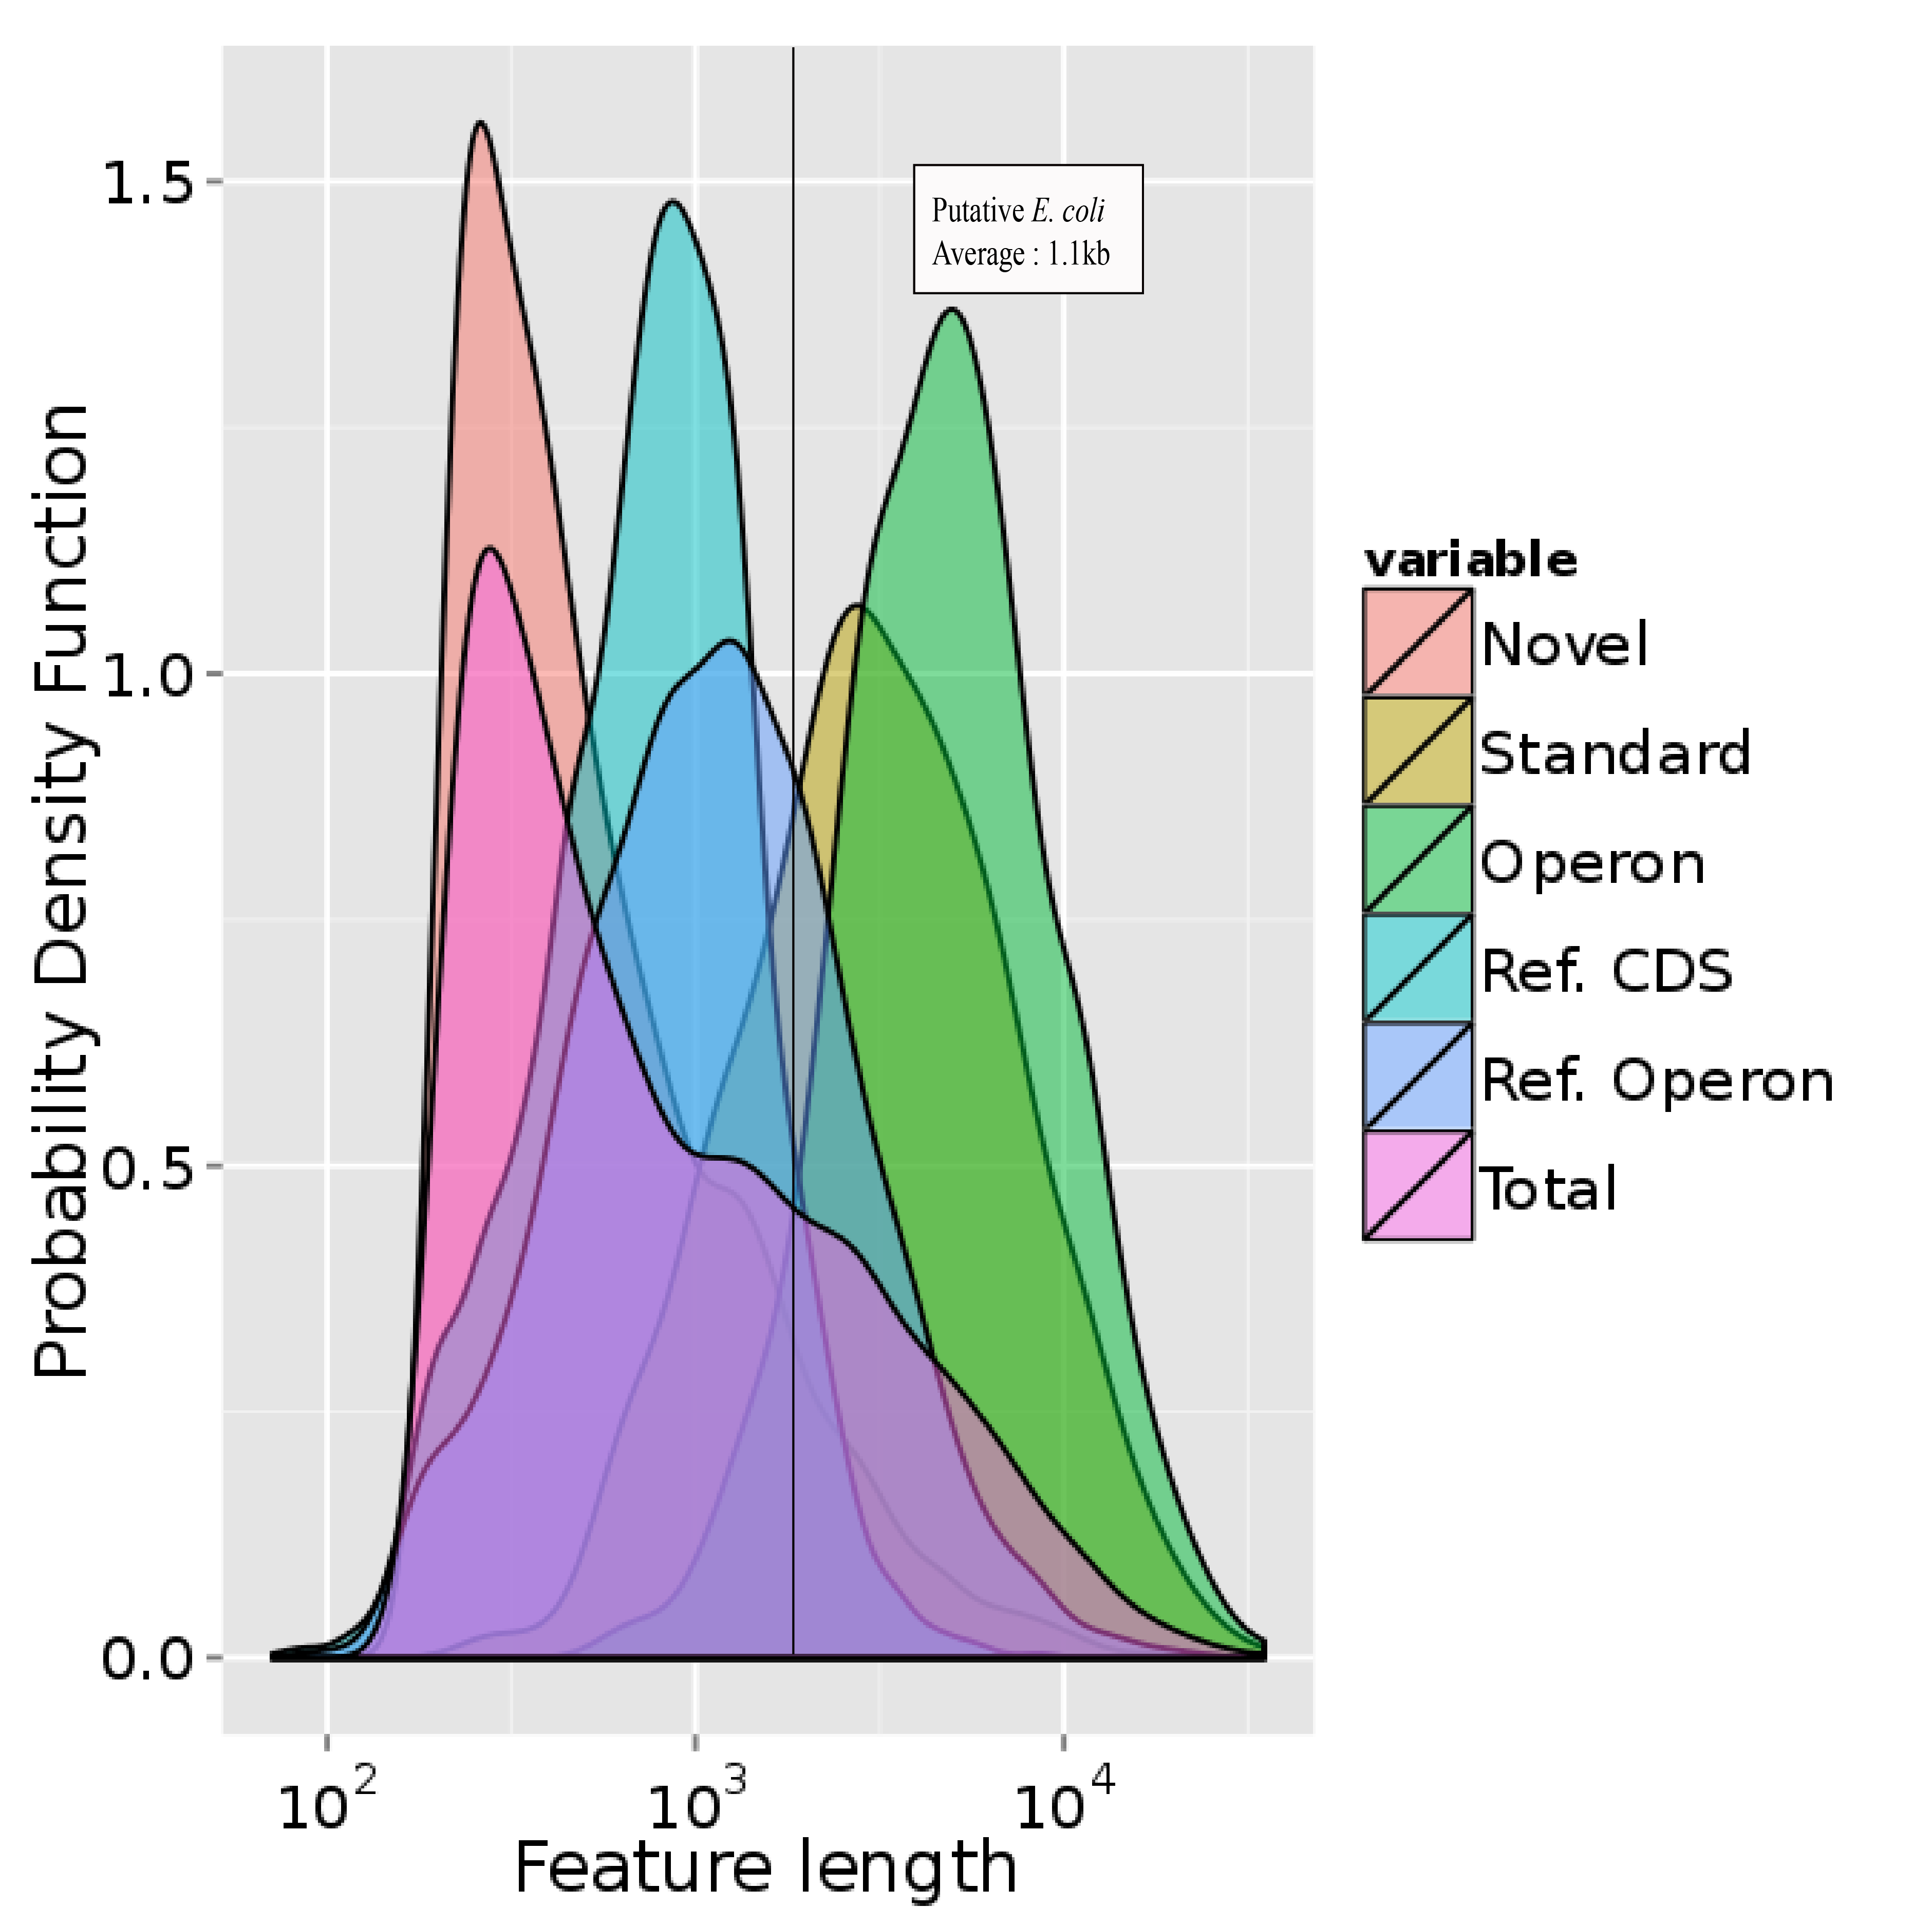
\includegraphics{images/Assembly/Summary/ffeature_length_1.png}
}
\end{minipage}
\end{center}
\caption{Transcript and Feature Length Distributions}
\end{figure}

\end{comment}




\subsection{Example Transcripts}


To assess the data/assembly quality further, I used canonical transcripts of \textit{C. acetobutylicum}, to understand the agreement of the coverage, the assembly, and the existing annotation. Six issues, listed below, were considered for each example to better understand the quality of the assembly and the degree of curation required. 

\begin{enumerate}
\item Is the transcript large enough to include the known ORFs and RBSes?
\item Does the assembled transcript's TSS agree with promoter motifs?
\item Does it agree with published transcription start sites?
\item Does the assembled transcript's size agree with published Northern blots?
\item Does the assembly represent the coverage and if not, which of these two best represents the biological knowledge of this region?
\item Does the assembled region require curation (e.g. fused, extended, or truncated transcripts)?
\end{enumerate}

Agreement between the data and the literature would support the efficacy of this technique. Its effectiveness is particulary important in cases where no previous experimental data exists. These results could be very useful to future studies if only minimal remediation or curation is required. The first example that I examine is the Sol locus.

\subsubsection{Sol Locus}

The Sol locus is a 7kb region on the pSol1 megaplasmid surrounding the Sol operon(4.3kb, basepairs 175,564-179,841). This region is responsible for the production of several solvents\cite{62,63}. This region encodes several enzymes including a tri-functional NAD(H\textsuperscript{+})-dependent alcohol/aldehyde dehydrogenase (AdhE)\cite{62}, two subunits of coenzyme-A transferases (ctfA/B)\cite{66}, and an acetoacetate decarboxylase (Adc)\cite{64,65,66}. The region is also home to a protein SolR, which includes a helix-turn-helix motif and is thought to regulate solventogenesis\cite{67}. These genes are vital for carboxylic acid reuptake and conversion into alcohols, a vital part of this organism's metabolism and the solventogenesis process.

%          SOL LOCUS Fig 1.
\begin{figure}
\small
{\includegraphics[width=\textwidth,height=2.5in]{images/Assembly/Examples/Sol/Curated-Sol-locus.png}
\subcaption{Sol locus}\label{fig:1a}}
% \label{fig:1}
\caption{Sol Locus Overview} This operon (\subref{fig:1a}) upper track) consists of OrfL, alcohol dehydrogenase (AdhE), and Co-A transferases A and B (ctfA,ctfB). SolR (far left) and acetoacetate decarboxylase (ADC; \subref{fig:1a} lower track, right) are also shown. Coverage for the Watson and Crick strands (top and bottom tracks) are visualized with an annotation track (center). Tracks show cumulative coverage for unstressed (yellow), butanol (light green/ light orange), and butyrate (green/orange) stressed samples over all time points. Transcripts (blue), ORFs (orange), RBSes (purple), inverted repeats (yellow), promoters (green), and TSSes (red) are represented as arrows and bars.
\end{figure}

\paragraph{Acetoacetate Decarboxylase Transcript}
In the early 1990s, several articles were published about the Sol locus including the cloning and sequencing of Adc and the Sol locus\cite{62,63,64,65,66}. An early study of the Sol operon probed the Adc locus, reporting two transcript sizes of 670 and 865 with Northern blot\cite{65}. The authors also reported the major transcription start site of Adc at base 180671 of the pSol1 plasmid. To examine the quality of our data and raw assembly, we examined this locus to observe the transcript size and locate the transcription start site in our data. In \ref{fig:2a} we see the transcription start site reported by Durre(red) located very near a sustained increase in sequencing coverage just downstream of a canonical promoter motif. This pattern of coverage (cumulatively \textgreater 10,000x) is sustained until a bidirectional Rho-independent terminator (\ref{fig:2b}). In this instance, the precise transcription start site was not estimated precisely by the uncurated assembly. The reported transcript continues for several hundred basepairs upstream of the Adc TSS, despite the decrease in coverage. This artifact is most likely due to sufficient k-mer complexity in the reads mapping upstream of the TSS for the Adc transcript to be fused to signal from genes upstream. Correcting for this error (\ref{fig:2c}), the full transcript size is 857. It was claimed that the 670bp product is most likely a specific degradation product or the result of a secondary transcriptional start site\cite{65}. To investigate this, a transcript of this size would correspond to a transcriptional start site at approximately base 180,484. Unfortunately, none of the promoter motifs in the region could explain a transcript of this size in vegetative cells. After curation based on the coverage pattern, promoter and terminator motifs in this region, the transcription start site and transcript size for Adc accurately match previous results. 

\begin{figure}
\small
{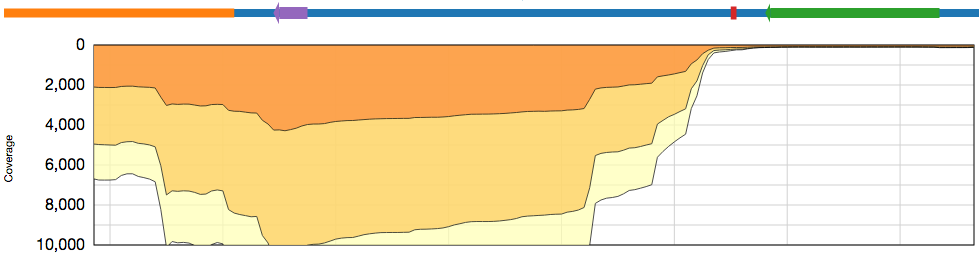
\includegraphics[width=\textwidth,height=1.5in]{images/Assembly/Examples/Sol/Sol-Adc-TSS.png}
\subcaption{Adc transcription initiation region on the Crick strand.}\label{fig:2a}}
{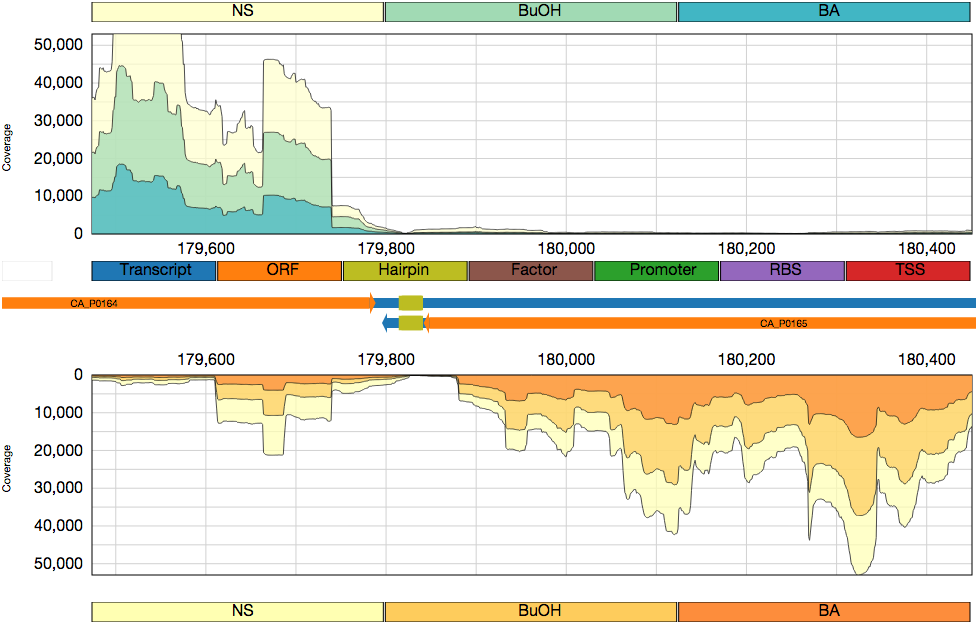
\includegraphics[width=\textwidth,height=2.5in]{images/Assembly/Examples/Sol/Sol-bifunctional-terminator.png}
\subcaption{Bifunctional Rho-independent terminator for Sol operon (upper track, left), Adc}\label{fig:2b}}
{\includegraphics[width=\textwidth,height=1.5in]{images/Assembly/Examples/Sol/Sol-Adc-curated.png}
\subcaption{Curated Adc locus}\label{fig:2c}}
\caption{Adc locus}
\subref{fig:2a}) Transcription initiation region for Adc. While the coverage clearly shows the appropriate increase, the transcription start site has been fused to residual coverage upstream of the true TSS. \subref{fig:2b}) A bifunctional terminator is responsible for transcriptional termination of both Adc and the Sol operon. \subref{fig:2c}) With minor curation, the region matches previous results faithfully.
\label{fig2}
\end{figure}


\paragraph{Sol Operon}
These studies additionally describe the Sol operon. In \cite{65}, Durre et al. examined the Sol operon using a probe specific for ctfB and reported a transcript size of 4.1kb. Unfortunately, no blots were included as figures in this work. In \cite{63} AdhE-based probes revealed a nearly identical transcript size of 4.1-4.2kb. Interestingly, the Sol operon has both proximal and distal transcription start sites at 175,726 and 175,564, respectively\cite{62,63}. Ribosome binding sites have been identified upstream of AdhE, CtfA, and CtfB\cite{63}. The expression level of the Sol operon is substantial, also upwards of 10,000x coverage cumulatively. The distal transcription start site is matched perfectly (\ref{fig:3a}), demonstrating the precision of the assembly technique in the absence of background or residual signal. An increase in coverage is observed immediately following the proximal promoter (\ref{fig:3a}) in close agreement with the previous determinations\cite{62,63}. However, the transcription stop site was not precisely determined by the assembly, owing in part to basal antisense signal from the Adc gene (\ref{fig:2b}). After adjustment, the transcript sizes are 4,115 and 4,277, respectively, in close agreement with the reported transcript sizes\cite{63,65}.

\begin{figure}
\small
{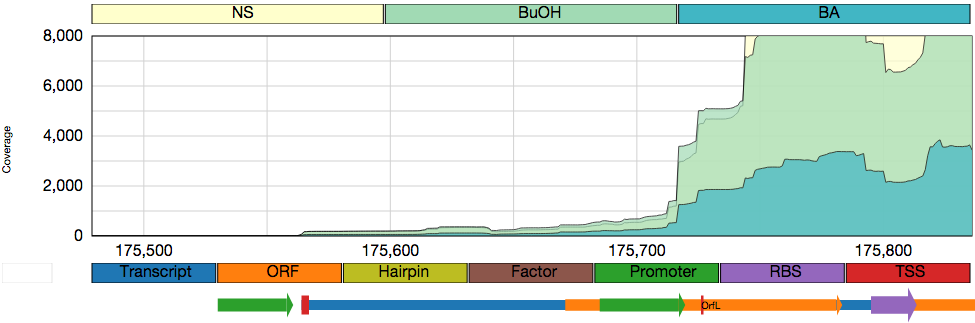
\includegraphics[width=\textwidth,height=1.5in]{images/Assembly/Examples/Sol/Sol-TSS.png}
\subcaption{Sol operon transcription initiation region. The distal (left) and proximal (right) transcription start sites (red) are shown for AdhE (far right, orange).}\label{fig:3a}}
{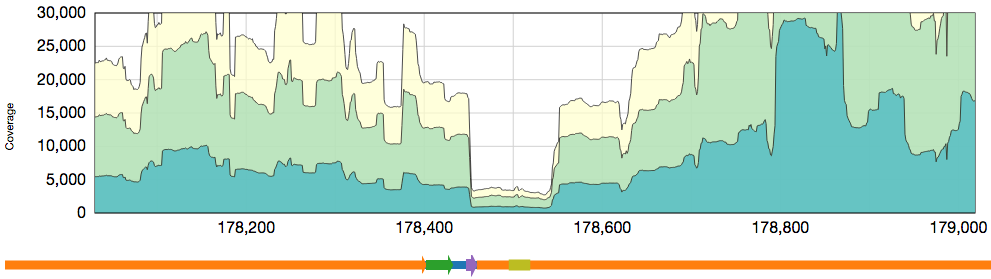
\includegraphics[width=\textwidth,height=1.5in]{images/Assembly/Examples/Sol/Sol-AdhE-terminator.png}
\subcaption{Putative AdhE (left) terminator, CtfA (right) promoter}\label{fig:3b}}
\caption{Sol Operon}
\subref{fig:3a}) Sol operon (OrfL, center; AdhE right) transcription start sites. The coverage and assembly data have strong agreement with previously described proximal and distal promoters and transcription start sites. \subref{fig:3b}) Low coverage in the Sol operon. A terminator may be partially responsible for a sustained low coverage level in the Sol operon. Additionally, a promoter motif was located upstream of the CtfA RBS and the pattern of expression is consistent with these observations.
\end{figure}

\paragraph{Multiple Transcripts from Sol Operon}
While the results from this region agree as a whole, there is an interesting pattern in coverage in the Sol operon near the C-terminus of AdhE(\ref{fig:3b}. This 100bp region is expressed at a statistically lower level (K.S.-test, p < 0.05) than the rest of the Sol operon. Upon further examination of this region, we find a Rho-independent terminator with a \(\Delta\)G of -9.6 kcal/mol, which is not as strong as the -11.5 kcal/mol bifunctional terminator at the end of the Sol operon. The region is also near a Sigma-A promoter motif of TTCATA(13)TATAAT located upstream of the previously mentioned RBS. As mentioned above, no Northern blots figures were included in the only study, to the best of my knowledge, that uses ctfA or ctfB specific probes\cite{65}. Most studies of the Sol operon in \textit{C. acetobutylicum} use AdhE-specific probes or larger restriction digestion probes \cite{63,68,70}. One of these displays a Northern with a weak but distinct band for a ~2.6kb transcript under solventogenic conditions \cite{68}. If AdhE were transcribed both in the classical Sol operon and as a separate transcript, the length would be 2,716bp from the proximal transcription start site. This pattern of coverage is consistent across all replicates. This length of the pattern suggests this observation does not merely represent difficulty sequencing secondary structure in the Sol operon transcript. In addition to the full Sol operon transcript, additional transcripts from the AdhE and ctfA/B genes may be produced.


\paragraph{SolR Transcript}
The last transcript produced from the Sol locus considered here is that of the SolR gene. This gene produces two transcripts, one 1kb and the other 1.3kb\cite{63}. A later study revealed the role of SolR as a repressor for the Sol operon\cite{67}. This study also produced a single transcription start site at 174,154 on the pSol1 plasmid. As a result of examining this dataset, we see a perfect recapitulation of the transcription start site (\ref{fig:4a}). The transcript from the raw assembly is approximately 1.2kb, showing only residual coverage (cumulatively \textless 5x) after the first terminator. After curation (\ref{fig:4b}), the transcript size is 1,036bp. There was insufficient coverage in the conditions studied to strongly support the larger transcript and no alternative transcription start sites were apparent.


% Transcription start sites SolR
\begin{figure}
{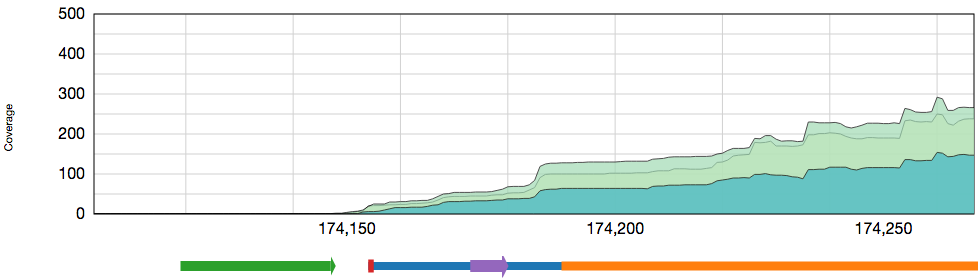
\includegraphics[width=\textwidth,height=1.5in]{images/Assembly/Examples/Sol/Sol-SolR-TSS.png}
\subcaption{SolR transcription initiation region}\label{fig:4a}}
{\includegraphics[width=\textwidth,height=1.5in]{images/Assembly/Examples/Sol/Sol-SolR-curated.png}
\subcaption{Curated SolR Transcript}\label{fig:4b}}
%\label{fig:1.5}
\caption{SolR Locus}
\subref{fig:4a}) The assembled transcription start site for SolR agrees with previous findings. \subref{fig:4b}) The curated SolR transcript agrees with previously published findings\cite{63,67}.
\end{figure}

\subsubsection{Bdh Locus}
The Bdh locus encodes two homologous butanol dehydrogenase(BDH) enzymes in a 3kb region on the main chromosome. Early studies of butanol dehydrogenases in \textit{Clostridia} located a number of NADH-dependent and NADPH-dependent BDHs and ADHs responsible for butanoate metabolism\cite{69,70,71,72}, specifically the reduction of butyryl and acetyl groups into the solvents butanol and ethanol. One such locus in \textit{C. acetobutylicum} produces two isozymes with different physiological roles. These isozymes like have distinct regulation and physiological roles from the other alcohol dehydrogenases found in this organism. The Bdh locus proteins were described by several authors, reporting different activities and specificities for each enzyme\cite{69,70}. After characterizing the enzymes in this locus, the region was cloned and two homologous isozymes were found. The two transcripts originating from these isozymes will demonstrate the precision and accuracy of this technique when compared to primer-extension analyses but also the need for assembly curation that reflects the motifs and coverage pattern of the region. We begin by discussing the first of these, BdhA.
\paragraph{BdhA}
BdhA is an NADH-dependent butanol dehydrogenase that acts on both butyryl and acetyl groups. Studies suggest that this enzyme has fairly comparable activities with both substrates, with slightly higher activities for butyryl groups\cite{70}. This enzyme was observed to have higher activities at low pH, indicative of its physiological role in the conversion of butyric acid to butanol. The entire locus was sequenced, producing ORFs that exactly matched the BdhA and BdhB isozymes\cite{72}. Northern analysis determined that these genes are transcribed separately and not as an operon. BdhA was found to have a 1.3kb transcript and the transcription start site was mapped through primer-extension to base 3,465,240 on the main chromosome of \textit{C. acetobutylicum}\cite{72}. Here we find the transcription start site of BdhA one base upstream at 3,465,241. The results of transcription start site identification agree well with the upstream Sigma-factor A promoter and the aforementioned start site. The uncurated assembly produces a transcription stop site at base 3,464,329, before the stop codon(\ref{fig:5b}). The pattern of coverage, however clearly reflects the Rho-independent terminator nearby. The final transcript reflects the assembly, coverage pattern, and motifs in this locus, agreeing with the transcription start site and a transcript length of 1,282bp. In this example, the fairly obvious coverage pattern was not reproduced by the assembly, demonstrating the need for some simple curation, integrating knowledge of previous experimental data and global predictions of promoter and terminator motifs with the coverage pattern and assembly.
%        B d h A
\begin{figure}
{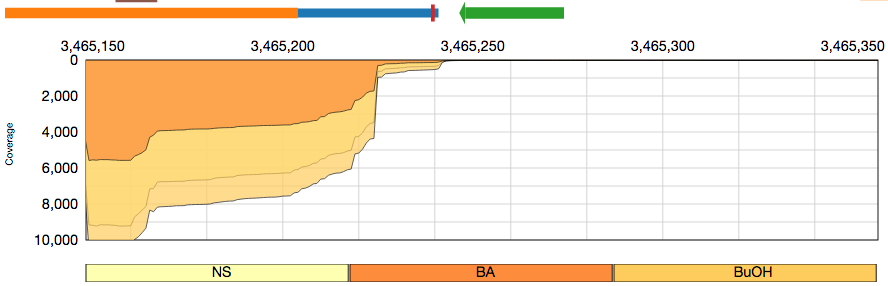
\includegraphics[width=\textwidth,height=1.5in]{images/Assembly/Examples/Bdh/BdhA-TSS.png}
\subcaption{BdhA Transcription Initiation Region}\label{fig:5a}}
{\includegraphics[width=\textwidth,height=1.5in]{images/Assembly/Examples/Bdh/BdhA-stop_site.png}
\subcaption{BdhA Transcription Termination Region}\label{fig:5b}}
{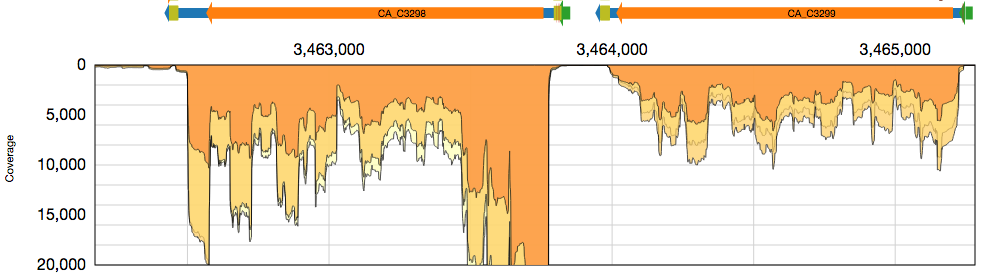
\includegraphics[width=\textwidth,height=1.5in]{images/Assembly/Examples/Bdh/Bdh-curated.png}
\subcaption{Curated BdhA Transcript}\label{fig:5c}}
\caption{Bdh Locus}
\subref{fig:5a}) The BdhA transcript displays a sharp increase in coverage near the transcriptional start site. This data agrees to a good extent with primer extension studies for this gene. \subref{fig:5b}) The raw assembly has failed to recapitulate the transcription termination region, likely due to low complexity coverage of the 3' region of this transcript. \subref{fig:5c}) The curated transcript reflects experimental characterization of this transcript\cite{72}.
\end{figure}

\paragraph{BdhB}
The next gene is BdhB, another NADH-dependent butanol dehydrogenase, with a slightly longer transcript size of 1.35kb. It was reported that this enzyme has 46-fold higher activity with butyryl groups than acetyl groups\cite{70,72}. BdhB was sequenced an analyzed along with BdhA, where it was discovered that BdhB had at least two transcription start sites, independent from BdhA. The most dominant transcription start site was very close to a secondary band at approximately 3,463,816 and 3,463,811, respectively\cite{72}. I will refer to these two distal bands collectively as the primary transcription start site for BdhB. A third band was located slightly farther upstream at 3,463,803\cite{72}. The coverage pattern for this region shows at least 3 sites of substantial increases in coverage at 3,463,802, 3,463,813, and 3,463,843 (\ref{fig:6a}). The first and proximal site has a promoter motif upstream, corresponding to the 1$^{st}$ -10 and -35 boxes in \ref{table:1} and the tertiary transcription start site\cite{72}. The second site has a significant increase in coverage between residue 3,463,817 and 3,463,810, which match well with the primary transcription start site described above\cite{72}. The primary transcription start site is explained by the 2$^{nd}$  -35 box and the 2$^{nd}$ or 3$^{rd}$ -10 box motifs\cite{72}. The final (distal) increase in coverage agrees with the 4$^{th}$ promoter motif(\ref{table:1}). It is clear that the strongest start site is the primary transcription start site previously described\cite{72}, although the multiple bands observed in their analysis could indeed be explained by matches to consensus Sigma-factor A motifs. Additionally, an observable but insignificant increase correlated with a final promoter motif. It is clear that the raw data match previous results to a good extent but curation was required to correct the transcription start site(\ref{fig:6a}) and stop site (\ref{fig:6b}). The final transcript is shown in \ref{fig:6c} with a final length of 1,367bp or 1,381bp, in close agreement with the published length of 1.35kb.

\begin{table}
\caption{BdhB Sigma-factor A boxes}\label{table:1}
\begin{minipage}[b]{2.5in}
\begin{center}
\begin{tabular}{|c|c|c|c|c|}\hline
\multicolumn{5}{c}{-35 box}\\\hline
Motif & Start & End & Sequence & p-value\\\hline
1 & 3463831 & 3463836 & TAGGTT & 3.5\e{-2}\\
2 & 3463847 & 3463852 & TTGTAA & 9.4\e{-3}\\
3 & 3463870 & 3463875 & TGGATA & 2.6\e{-2}\\\hline
\end{tabular}
\end{center}
\end{minipage}
\begin{minipage}[b]{2.5in}
\begin{center}
\begin{tabular}{|c|c|c|c|c|}\hline
\multicolumn{5}{c}{-10 Box}\\\hline
Motif & Start & End & Sequence & p-value\\\hline
1 & 3463816 & 3463821 & TATAAT & 4.3\e{-4}\\
2 & 3463820 & 3463825 & TATATA & 1.6\e{-3}\\
3 & 3463830 & 3463835 & TAAAAT & 4.2\e{-3}\\
4 & 3463852 & 3463857 & TATTAT & 4.2\e{-3}\\\hline

\end{tabular}
\end{center}
\end{minipage}
\end{table}
\begin{figure}
\small
{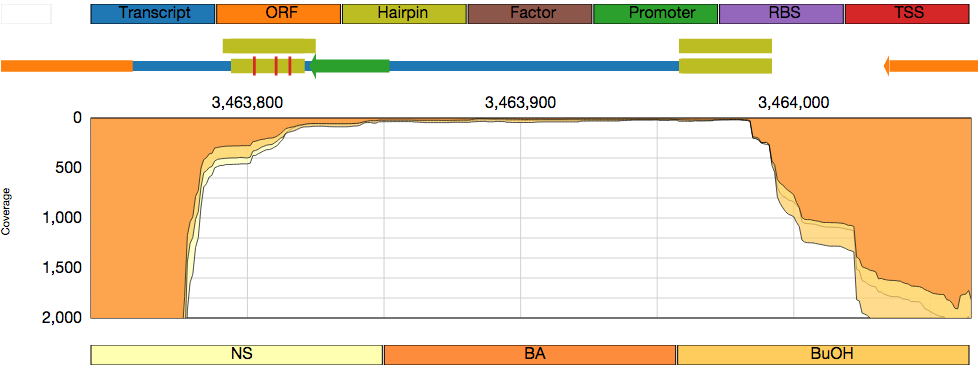
\includegraphics[width=\textwidth,height=1.5in]{images/Assembly/Examples/Bdh/BdhB-TSS.png}
\subcaption{BdhB Transcription Initiation Region}\label{fig:6a}}
{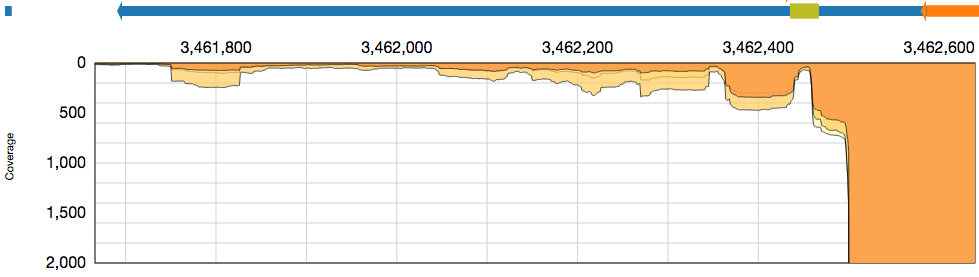
\includegraphics[width=\textwidth,height=1.5in]{images/Assembly/Examples/Bdh/BdhB-termination.png}
\subcaption{BdhB Transcription Termination Region}\label{fig:6b}}
{\includegraphics[width=\textwidth,height=1.5in]{images/Assembly/Examples/Bdh/BdhB-curated.png}
\subcaption{Curated BdhB Transcript}\label{fig:6c}}
\caption{Bdh Locus and Transcription Start Sites}
\subref{fig:6a}) The BdhB transcript has several promoter motifs and matching increases of coverage. These increases agree with previous experimental results\cite{72}, 2 of which were dismissed after not identifying the appropriate promoters. Unfortunately, the transcription start site was incorrect in the raw assembly. \subref{fig:6b}) A Rho-independent terminator is found at the end of the BdhB transcript although residual coverage triggered misassembly. \subref{fig:6c}) The final transcript matches previous results after integrating promoter and terminator motif information with the coverage pattern and assembly.
\end{figure}

In this example, the BdhA and BdhB transcripts were very close to capturing the true boundaries of these genes. In the case of BdhA the TSS was precise, but the assembled transcript did not match the coverage pattern or the ORF and terminator annotations. In the case of BdhB however, the start and stop sites did not agree with patterns in coverage and were simple to correct. The next example is another positive example, this time of a stress-response operon containing the heat-shock proteins GroES and GroEL.

\subsubsection{GroES/EL Locus}
\paragraph{GroES/EL Operon}
The GroES and GroEL proteins are evolutionarily conserved heat-shock responsive chaperonins. These proteins are found throughout the tree of life, including \textit{C. acetobutylicum}, where they are an integral to the solvent stress response\cite{73,74,75} and the class I heat-shock response\cite{42,73,74}. Expression levels are both strong and constitutive for this region, with a dramatic and transient increase with solvent or heat stress\cite{73,74}. In a molecular study, GroES and GroEL were found to be produced from a bicistronic operon with a transcript size of 2,150bp\cite{75}. In addition, a Sigma-factor A promoter was identified for an experimentally determined transcription start site. Two bands were observed during the primer-extension assay\cite{75}. The proximal band was dismissed as an artifact although the bands persisted under all conditions examined\cite{75}. This region is known to contain at least one CIRCE motif upstream\cite{76} and one overlaps both of these start sites (\ref{fig:7a})\cite{74}. The transcription start site determined in this work is located at 2,829,142, a mere two bases away from the previously reported start site\cite{75} (\ref{fig:7a}). Interestingly, the second transcription start site is located at a sharp increase in expression. The distance of this start site from the promoter suggests post-transcriptional processing. The transcription stop site is located near a Rho-independent terminator (\ref{fig:7b}). The transcript size determined by the raw assembly is 2,131bp in agreement with the 2.2kb band and the 2,150bp calculated distance between the transcription start-site and the Rho-independent terminator\cite{75}. In this example, the uncurated assembly produced a flawless recapitulation of the coordinates and size of the GroES/EL operon (\ref{fig:7b}). Having established the coordinates for this transcript in agreement with previous findings, the regulation of this operon should be briefly discussed.

\paragraph{GroES/EL Regulation}
The GroES/EL operon is stress responsive, although its expression under stress appears lower in \ref{fig:7c}. For this reason, it is worth discussing the regulation of this region and why these results are consistent with knowledge of this area. The CIRCE motif upstream of GroES is regulated by HrcA, a heat responsive repressor\cite{42,76,77}. In response to heat-shock, the GroES/EL operon is derepressed, revealing a Sigma factor A promoter and resulting in transcription (\ref{fig:7a}). The response to heat shock is fairly acute, increasing for 2-3 minutes and returning to standard levels after an additional 10 minutes\cite{76}. Here a general decreased expression is observed in response to solvent stress for two reasons. First, the 6S small RNA is a stress and growth-stage responsive regulator that globally reduces transcription from Sigma factor A promoters\cite{39,78}. Additionally, the time scale assessed here does not include a 3 minute time-point to identify an acute stress response. The stress response observed is the global downregulation of Sigma factor A promoters and the transition of the transcriptome towards one designed to tolerate stress. Sigma factor A dependent promoters are downregulated throughout this dataset as a result of the 6S small RNA. For this reason, we defer the test of differential expression for these time points for the next chapter. In the case of the GroES/EL operon, we observe precise and accurate estimates of transcript boundaries from the uncurated assembly. Additionally, we observe the effect of a complicating factor in differential analysis: the effect of the 6S small RNA on Sigma A dependent promoters at the time scales we are analyzing. The next example is the regulator responsible for the acute stress response of these heat shock proteins, HrcA.


\begin{figure}
\small
{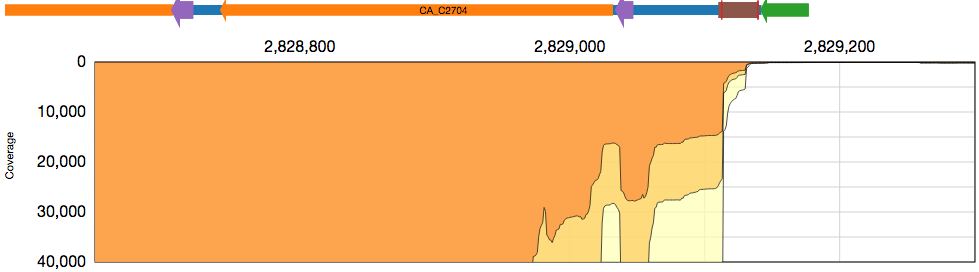
\includegraphics[width=\textwidth,height=1.5in]{images/Assembly/Examples/GroESL/GroESL-TSS.png}
\subcaption{GroES/EL Transcription Initiation Region}\label{fig:7a}}
{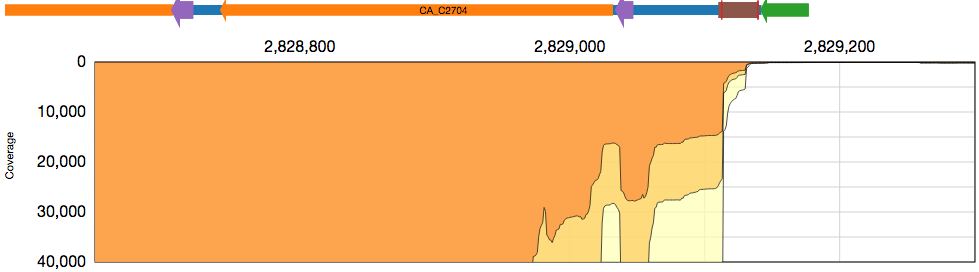
\includegraphics[width=\textwidth,height=1.5in]{images/Assembly/Examples/GroESL/GroESL-TSS.png}
\subcaption{GroES/EL Transcription Termination Region}\label{fig:7b}}
{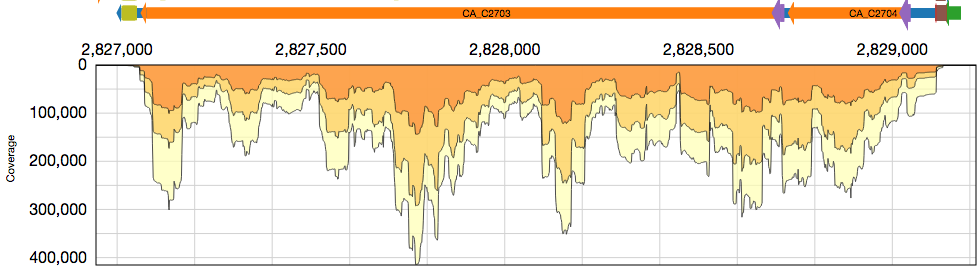
\includegraphics[width=\textwidth,height=1.5in]{images/Assembly/Examples/GroESL/GroESL-curated.png}
\subcaption{GroES/EL Locus}\label{fig:7c}}
\caption{GroES/EL Locus}
\subref{fig:5a}) GroES and GroEL form an operon that is responsive to heat-shock through a HrcA-mediated derepression mechanism. The transcription start sites are in agreement with previous findings with the addition of an interesting peak inbetween these two. \subref{fig:5b}) The transcription termination region supports previous reports of a 2.2kb transcript terminating at a Rho-independent terminator following the GroEL ORF.
\end{figure}

%   H r c A,  G r p E,  D n a K,  &  D n a J
\subsubsection{HrcA and DnaK/J Locus}
\paragraph{DnaK Locus Overview}
This rather complex locus encodes the class I repressor HrcA and DnaK and DnaJ, another set of evolutionarily conserved heat-shock proteins. DnaK was discovered to be solvent-stress responsive in \textit{C. acetobutylicum}\cite{73,74}. Solvent stress and heat shock increase protein denaturation, requiring molecular chaperones such as GroES/EL and DnaK/J to increase proper protein folding in these conditions. The \textit{C. acetobutylicum} DnaK protein was purified as a stress responsive 74kDa protein\cite{74}. Using a restriction fragment, the DnaK locus was then cloned and sequenced\cite{79}, revealing a grouping of four ORFs, similar in arrangement to \textit{B. subtilis}\cite{76}. An inverted repeat, now known to be the HrcA-binding CIRCE motif, was found upstream of the HrcA gene\cite{79}. Upon Northern analysis of this region, three different transcripts were identified as originating from this locus, of 2.6, 3.8, and 5kb lengths. Additionally, a 1.5kb band was observed with a DnaK specific probe\cite{79}. The first transcript (2.6kb) could be seen with a DnaK-specific probe and is thought to contain the genes GrpE and DnaK. The second transcript (3.6kb) was observed for both DnaK and HrcA-specific probes and is thought to contain the same genes plus HrcA. Similarly, the 5kb transcript was observed for both probes and is thought to contain the whole operon. The final transcript(1.4kb) and additional small bands were dismissed as specific degradation products. It has been noted that this operon has interesting post-transcriptional regulation in \textit{B. subtilis}, producing multiple transcripts from a heptacistronic operon\cite{82}. To analyze this complex operon, we will proceed through 4 proposed regulatory sites. The first is the promoter region of HrcA. The second site is a transcription start site upstream of GrpE. The third is the location of an internal CIRCE motif, terminator, and an additional transcription start site ahead of DnaJ. The final site is located at the end of the whole operon.

\paragraph{HrcA Promoter}
The HrcA promoter was described during the sequencing of the DnaK/J locus\cite{79}. This promoter produces the full transcript of 5kb and the smaller 3.6kb transcript terminating between DnaK and DnaJ. Two transcription start sites have been described for this region\cite{79}. Both of the two reported transcription start sites(S1 and S2) were located upstream of the CIRCE element, in contrast to groES/EL (\ref{fig:8a}). Additional bands present in the primer extension analysis were rejected similarly to the strand bands in the GroES/EL operon. An excellent Sigma factor A motif was located for the S1 site (P1,\ref{table:2}) but only an insignificant motif (p > 0.05, TTTATG(17)AAAGAT) motif was found for the weak band of the S2 site. An alternative promoter (P2, \ref{table:2}) seems to be too close to the S2 transcription start site. If the observed bands represent true transcription start sites for this operon they are transcribed from close and overlapping promoter motifs. Here we don't see any direct increase in transcription for the S1 site, most likely due sequencing difficulty near the CIRCE motif. Upon TEX enrichment, no increase or decrease in coverage can be observed near these sites, suggesting that post-transcriptional processing is not responsible for these transcription start sites. The increases in transcription observed here are relatively minor compared to the transcription of the entire HrcA operon. The P1 and P2 motifs seem to be sufficient for transcription initiation, although the coverage pattern shows evidence of complication of sequencing. In several studies\cite{75,79} transcription start sites have been discarded due to local RNA secondary structure. It is reasonable that reverse transcription in this area may be complicated by the -10kcal/mol hairpin and CIRCE motif near the 5' end of the transcript. Several authors have noted that full HrcA/DnaK operon transcripts are present at lower abundance\cite{79,82}, resulting in lower coverage and an indistinct transcription start site when considering coverage alone. In \ref{fig:8a}, it is clear that the uncurated assembly estimated the transcription start site more accurately than a coverage-only approach would provide. As we have seen, in some cases the De-bruijn graph assembly requires curation to most accurately reflect local motifs. On the other hand, this method produces a reasonable estimate of the start site. After minor curation, the transcription start site agrees with the previously described\cite{79} S2 and S1 (\ref{fig:8b}). Having established the transcription start site for the entire HrcA operon and previous transcriptional start sites are not the result of post-transcriptional processing, we move on to the higher abundance transcripts produced by this region, beginning with the GrpE operon.

\paragraph{GrpE Promoter}
The GrpE protein is an essential nucleotide exchange factor for DnaK. This protein was discovered upstream of DnaK after cloning and sequencing of the DnaK locus\cite{79}. It was postulated that a second transcription start site upstream of GrpE would explain the smaller 2.6kb transcript and a transcription start site was determined\cite{79}. A transcription start site exists ahead of the GrpE gene in \textit{B. subtilis} as well\cite{82}. The proposed promoter ahead of GrpE does not match the Sigma factor A consensus (p > 0.05) and no alternative motifs were found. However, a substantial increase in coverage can be found further upstream from this site. The first two sites are specifically enriched in the TEX treated library, suggesting a transcription start site. Promoter motifs of higher quality are found upstream of two major peaks (\ref{fig:8b}). Looking at the entire operon (\ref{fig:8c}) it is clear that this is a substantial transcription start site. The increase in coverage here is acute in contrast with the previous site in the conditions of this study. Additionally, it has been proposed that the HrcA operon is generated from post-transcriptional processing and differing transcript abundances are due to differing decay rates\cite{82}. If such a processing mechanism were present in \textit{C. acetobutylicum}, the coverage at the GrpE transcription start site would be differential with respect to the 5'-phosphate exonuclease (TEX) treatment. In \ref{fig:8b}, the coverage is not differential at this or other locations in this transcript, demonstrating that the 2.6kb transcripts is most likely a primary transcript originating from the Sigma factor A promoters P3 or P4. In summary, a novel transcription start site and promoter motif were located upstream of GrpE. No matching promoter motif or coverage pattern was observed for a previously documented transcription start site under these conditions. Additionally, coverage at the novel transcription start site was enriched with TEX treatment, suggesting that the 2.6kb transcripts are primary transcripts and not products of post-transcriptional processing.CtsR and CIRCE motifs were not found near this transcription start site. Next, the DnaK/J intergenic region is explored, which contains a terminator responsible for read-through transcription of the entire 5kb operon.

\begin{figure}
{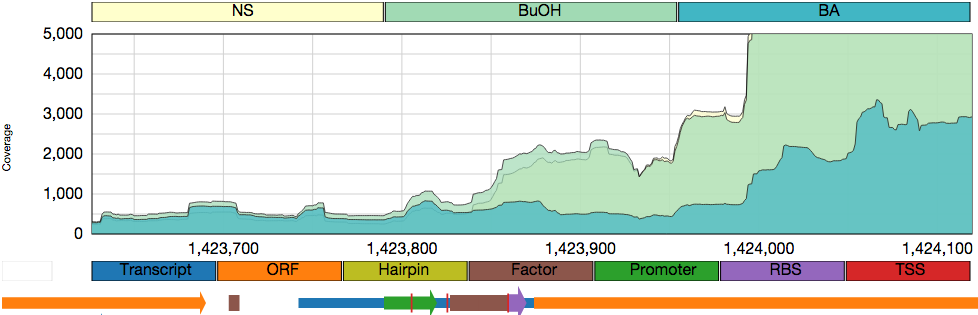
\includegraphics[width=\textwidth,height=1.5in]{images/Assembly/Examples/HrcA/HrcA-TSS.png}
\subcaption{HrcA Transcription Initiation Region}\label{fig:8a}}
{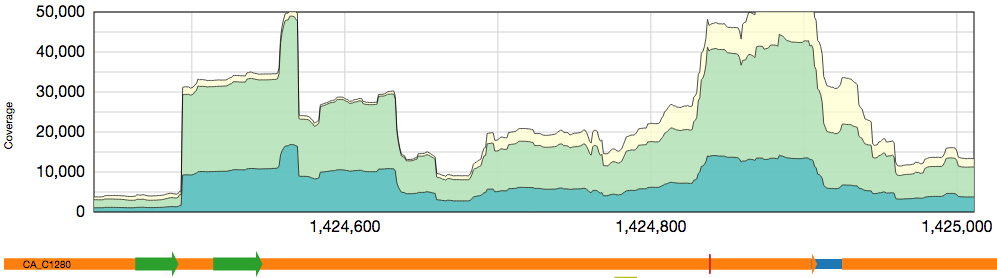
\includegraphics[width=\textwidth,height=1.5in]{images/Assembly/Examples/HrcA/GrpE-TSS.png}
\subcaption{GrpE Transcription Initiation Region}\label{fig:8b}}
{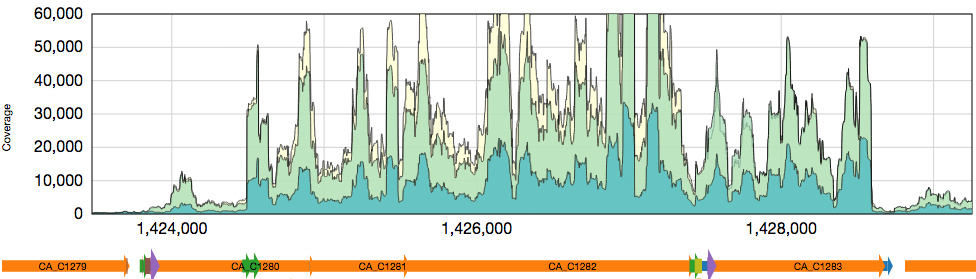
\includegraphics[width=\textwidth,height=1.5in]{images/Assembly/Examples/HrcA/HrcA-operon-curated.png}
\subcaption{Curated HrcA Locus}\label{fig:8c}}
\caption{HrcA Locus}
\subref{fig:8a}) HrcA leads the 5kb tetracistronic operon. The regulation of this operon consists of Sigma factor A dependent promoters, a CstR motif, and a CIRCE motif. \subref{fig:8b}) A secondary transcription start site in upstream of GrpE is responsible for the 2.6kb and 3.8kb transcripts. A large increase in coverage at a novel transcription start site is not TEX responsive. \subref{fig:8c}) The curated HrcA operon has two transcription start sites and one Rho-independent terminator which explain the 5kb, 3.8kb, and 2.6kb transcipts reported for this area.
\end{figure}


\begin{table}
\caption{HrcA Operon Sigma-factor A boxes}\label{table:2}
\begin{minipage}[b]{2.5in}
\begin{center}
\begin{tabular}{|c|c|c|c|c|}\hline
\multicolumn{5}{c}{-35 box}\\\hline
Motif & Start & End & Sequence & p-value\\\hline
P1 & 1423790 & 1423795 & TTGACA & 2.9\e{-4}\\
P2 & 1423774 & 1423779 & ATGAAA & 5.3\e{-2}\\
P3 & 1424463 & 1424468 & TTGAGG & 1.6\e{-2}\\
P4 & 1424514 & 1424519 & TTGATT & 6.2\e{-3}\\
P5 & 1427399 & 1427804 & TTGAAA & 2.1\e{-3}\\
\hline
\end{tabular}
\end{center}
\end{minipage}
\begin{minipage}[b]{2.5in}
\begin{center}
\begin{tabular}{|c|c|c|c|c|}\hline
\multicolumn{5}{c}{-10 Box}\\\hline
Motif & Start & End & Sequence & p-value\\\hline
P1 & 1423812 & 1423817 & TATTTT & 2.3\e{-2}\\
P2 & 1423800 & 1423805 & TAATGT & 1.8\e{-2}\\
P3.1 & 1424476 & 1424481 & TAATAT & 9.9\e{-3}\\
P3.2 & 1424482 & 1424487 & TAAAAA & 3.2\e{-2}\\
P4 & 1424537 & 1424542 & TATGAT & 1.9\e{-3}\\
P5 & 1427430 & 1427435 & TATAGT & 2.5\e{-3}\\\hline
\end{tabular}
\end{center}
\end{minipage}
\end{table}

\paragraph{DnaK/J Intergenic Region}
The DnaK/DnaJ intergenic region is known to contain a Rho-independent terminator\cite{79,82}, thought to be responsible for the 3.8kb and 2.6kb transcripts. The \(Delta\)G of this terminator is estimated to be -13.2kcal/mol. In \ref{fig:9a}, decreased coverage is observed near this terminator, upstream of the DnaJ gene. This terminator does not contain a CIRCE element, in contrast to the inverted repeat at the HrcA promoter. A strong promoter motif (P5,\ref{table:2}) is observed very close to a sharp increase in coverage at the 5' end of the repeat. The previously reported band is found on the 3' end of the repeat, which is explained by the strong terminator motif, similar to bands near the start of GroES/EL and HrcA. To my knowledge, no DnaJ-specific Northern blots have been produced to identify a 1.2kb monocistronic transcript and thus, whether the promoter and observed increase in coverage reflect a true transcription start site remains unknown. Suggested alternative explanations include post-transcriptional processing or thermodynamic challenges for the reverse transcriptase\cite{79}. However, the coverage pattern does not show a response to the TEX treatment (\ref{fig:9a}) and the former seems unlikely here. In the DnaK/J intergenic region, a decrease in coverage is observed near a strong Rho-independent terminator. Subsequently, increased coverage is observed near a strong promoter motif that might explain previous primer-extension results\cite{79}.


\paragraph{HrcA Transcript Termination}
The full operon is produced in a 5kb transcript which terminates after the DnaJ gene. In \ref{fig:9b}, a dramatic decrease in coverage is observed at the end of the DnaJ gene, 50 bases before the stop codon. Four terminator prediction software did not produce results for the transcription termination region shown here. This location should contain a non-intrinsic termination signal to explain the dramatic decrease in coverage. The residual signal from the nearby ribosomal methyltransferase(CA_C1284) matches well with evidence of a longer 8kb transcript in \textit{B. subtilis}\cite{82}. Given the dramatic decrease in coverage observed here, a reasonable transcription stop site for the 5kb operon can be assumed to follow the DnaJ gene(\ref{fig:8c}). Having discussed the regulatory regions of the HrcA operon, the final task is to summarize the transcript lengths, their regulation, and identify missing regulatory elements.


\begin{figure}
\small
{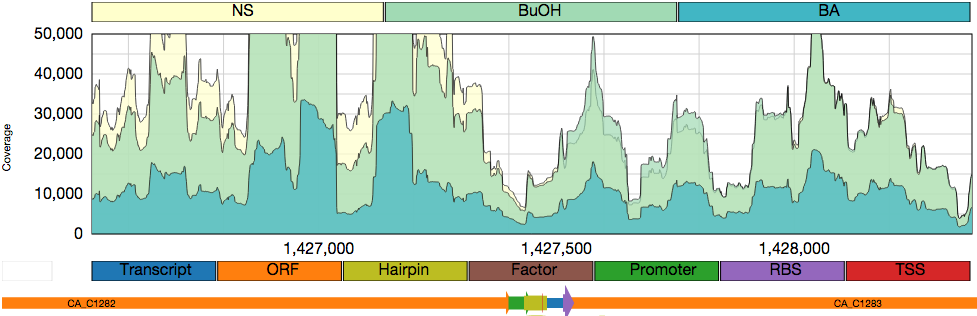
\includegraphics[width=\textwidth,height=1.5in]{images/Assembly/Examples/HrcA/DnaKJ-IGR.png}
\subcaption{DnaK/DnaJ Intergenic Region}\label{fig:9a}}
{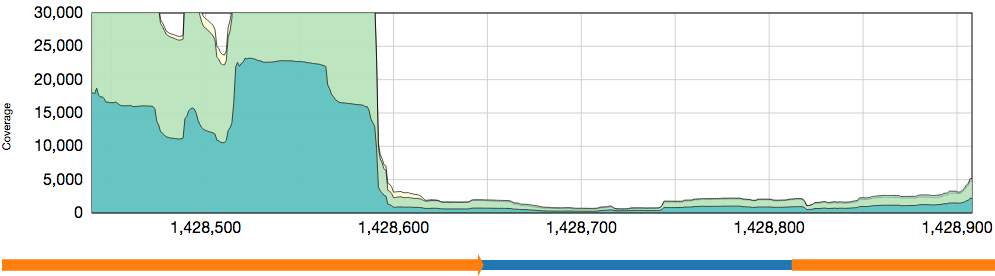
\includegraphics[width=\textwidth,height=1.5in]{images/Assembly/Examples/HrcA/HrcA-termination.png}
\subcaption{HrcA Transcription Termination Region.}\label{fig:9b}}
\caption{HrcA locus}
\subref{fig:9a}) The DnaK/DnaJ intergenic region consists of a Rho-independent terminator for the 2.6kb and 3.8kb transcripts. The coverage this region rebounds after a promoter motif and is not depleted with TEX treatment. \subref{fig:9b}) Near the end of the DnaJ gene, a dramatic decrease in coverage signals the end of the 5kb HrcA operon. No terminators can be found in this region, suggesting a non-intrinsic termination signal.
\end{figure}


\paragraph{HrcA/GrpE Transcript Lengths}
In the HrcA locus, two transcription initiation regions and two termination regions are responsible for 3 previously reported transcript sizes, 2.6, 3.8, and 5kb, respectively. The longest transcript observed here is 4,838bp from the HrcA transcription initiation region to the termination region downstream from DnaJ. The second largest observable transcript begins at one of the two start sites from the GrpE transcription initiation region and ends at DnaJ termination region, leading to transcripts between 3,778 to 4,125 bases, respectively. This region is the most abundant portion of this operon and may contain at least two smaller transcripts. The first of these species would begin at the GrpE transcription initiation region and terminate in the DnaK/J intergenic region. This type of transcript would range in size between 2,642bp and 2,989bp, respectively. The fourth and final transcript could originate from the DnaK/J intergenic region and terminate at the end of DnaJ, with a length of approximately 1.2kb. In the model organism \textit{B. subtilis}, larger transcripts are produced from this region, up to 8kb in length\cite{82}. It was observed that the transcripts and proteins of this region increase and decrease at different rates\cite{82}. Determining all the potential transcription start sites inside a region of continuous transcription is an ongoing challenge for understanding of the stress response. To conclude, the regulatory motifs and their locations in this region are summarized.

\paragraph{HrcA Locus Regulation}
Both Sigma factor A or H dependent promoters could be observed in the transcription initiation regions, as detailed above (\ref{table:2}). Sigma factor A promoters are under the control of the 6S small RNA, which has considerable expression in this study. Therefore, the activity of this locus must be considered with respect to global Sigma A promoter activity. Additionally, the HrcA transcription initiation region is under the direct control of both a CIRCE motif (3.2\e{-13}) and a CtsR motif (1.8\e{-7})\cite{42}. The inverted repeat in the DnaK/J intergenic region does not match either motif and is therefore most likely a Rho-independent terminator. The DnaJ termination region (+/- 200bp from the DnaJ stop codon) does not contain a detectable Rho-independent terminator and thus terminates transcription in a non-intrinsic manner, as previously suggested\cite{83}. The sequencing technique has produced excellent results for this region. The assembly produced a better estimate of the transcription start site than would be expected from coverage alone and a novel transcription start site was identified. Additionally, exact coordinates of regulatory motifs match well with the observed transcription start sites. Finally, potential transcript sizes were discussed to the extent permissible with this technique and the complexity of this region. Next, the Spo0A locus is considered an important gene in this organism that has not had the level of molecular investigation of the previous examples.




%          S p o 0 A
\subsubsection{Spo0A Locus}
\paragraph{Spo0A}
Spo0A is the master regulator of sporulation and stationary phase phenomena. This protein transduces growth-limiting and stressful signals into sporulation behavior in a number of firmicutes. In previous studies, Spo0A was shown to be translated from a 0.9kb transcript in \textit{C. acetobutylicum}\cite{84}. Additionally, a Sigma factor A and Sigma factor H motif were identified upstream of spo0A, but sadly neither the motifs nor the coordinates were provided. A single Sigma factor A motif (\ref{table:3}) was identified near a substantial increase in transcriptional activity (\ref{fig:10a}). A single Spo0A box was reported upstream of Spo0A\cite{84} and can be seen in \ref{fig:10a}. A single terminator motif is located ~130 basepairs downstream of the stop Spo0A stop codon. The uncurated assembly did not identify single start or stop sites for this gene, fusing Spo0A with signal on either side of the gene. After curation with these information combined, we observe a transcript of 1,147bp, longer than the 0.9kb transcript detected by Northern blot in a previous study of this locus\cite{84}. This represents the first documentation of the Spo0A transcript boundaries in \textit{C. acetobutylicum}.


\begin{table}
\caption{Spo0A Regulatory Motifs}\label{table:3}
\begin{minipage}[b]{2.5in}
\begin{center}
\begin{tabular}{|c|c|c|c|c|}\hline
\multicolumn{5}{c}{Sigma A}\\\hline
Motif & Start & End & Sequence & p-value\\\hline
-35 & 2173565 & 2173560 & TTGATT & 6.2\e{-3}\\
-10 & 2173537 & 2173542 & TAAAAT & 1.5\e{-3}\\
\hline
\end{tabular}
\end{center}
\end{minipage}
\begin{minipage}[b]{2.5in}
\begin{center}
\begin{tabular}{|c|c|c|c|c|}\hline
\multicolumn{5}{c}{Spo0A Box}\\\hline
Motif & Start & End & Sequence & p-value\\\hline
1 & 2173430 & 2173436 & TGTCGAA & 1.9\e{-4}\\
\hline
\end{tabular}
\end{center}
\end{minipage}
\end{table}


\paragraph{Missing from the Databases: CA_C2079}

In a nearby location, the genes CAC2073-2078 are found in a tight grouping near a large peak of expression. This peak correpsonds to an uncharacterized protein CAC2079 that is present in UniProt but absent from NCBI and KEGG databases. Its coverage appears to be largely above 20k per base, independent of the surrounding regions (although the transcript is indeed fused). Bioinformatic analysis suggests that it shares sequence similarity to proteins in the \textit{Clostridia}, \textit{Bacilli}, \textit{Baceteroidetes}, and \textit{Halobacteria}. While there was no common catalytic or active domain unifying this group of homologs, the region of homology tends to precede a transmembrane motif. Further analysis via PSI-blast result suggests sequence similarity to mATE (Multidrug And Toxic-compound Extrusion) efflux family proteins. mATE family proteins use electrochemical gradients to export antibiotics and other toxic compounds. The data suggest that the expression of this protein is important to \textit{C. acetobutylicum} and it will be interesting to examine the expression profile statistically. This example illustrates the synergy of this transcriptomic dataset with existing annotation and the benefit of curation. 


\subsection{Identify and Attempt to Resolve Remaining Issues}
There are two principal challenges relating to this uncurated transcriptome assembly. The first relates to the qualification of novel transcripts which I will defer to a later time. The second involves the curation of the 1057 transcripts which encode reference CDSes. After considering the examples above, we are left with a few types of misassembly to address.
\begin{enumerate}
\item Partial transcripts which overlap reference ORFs, but do not completely contain them. (e.g. BdhA)
\item Extended transcripts that possess larger UTRs than would be expected with respect to promoter and terminator motifs and coverage patterns. (e.g. Adc, CtfA/B)
\item Fused transcripts where the transcript from one gene is completely fused with signal from neighboring loci, with respect to prior knowledge, promoter, and terminator motifs (e.g. Spo0A).
\end{enumerate}

The first issue requires the simple solution of adjusting the transcript boundaries to include reference ORFs where there is not complete inclusion. Practically this requires only some minimal scripting and the use of '\href{http://bedtools.readthedocs.org/en/latest/content/tools/merge.html}{merge}' from bedtools, a toolkit for genomic set operations. The second issue requires a slightly more complicated solution of integrating information of regulatory motifs, terminators, and coverage information to find the solution that produces the most agreement between these various sources. In practice, I will integrate the various sources in the genome browser for context with the coverage information from this experiment. No completely automated tools exist to accomplish this. However, on average each transcript requires only a minimal amount of decision and should in principle be easy to curate. The third type of gene is completely fused to signal from other genes or noise. In the case of Spo0A, the true signal was simple to distinguish from noise, even in the absence of a Rho-independent terminator. In other cases the solution may not be so simple but contextual information about ontology combined with the various signals of coverage and stress response, promoters, and terminators make the problem more tractable. 

In principle, each of the pieces of information that I will integrate will not reproduce the transcript boundary on its own. In the examples above there are instances where the coverage alone fails to describe the transcript boundary, while the linguistic complexity of the dataset, used by the assembly algorithm, reproduces the boundary to a good extent. In other instances the opposite is true: a dramatic change in coverage near terminators or other signals is not recognized by the assembly alone. For that matter, there appear to be instances of non-intrinsic termination to complicate matters further. Therefore, these information are synergistic with respect to defining transcript boundaries and the absence of one signal may be made up for by the presence of another.

\subsection{Novel Transcripts}

\subsection{Exploratory Tools}


